%------------------------------------------------------
%
%   Mijenjati po potrebi, i to u vlastitom predavanju!
%
%   Za promjene u samom predlošku,
%   konzultirajte osobu zaduženu za održavanje.
%
%------------------------------------------------------

\documentclass[crop=false, class = scrartcl]{standalone}

\usepackage[utf8]{inputenc}
\usepackage[T1]{fontenc}
\usepackage[croatian]{babel}

\usepackage{mlmodern} % za fontove
 
\usepackage{csquotes} % za prave navodnike

\usepackage{subfiles} % da mogu različiti fileovi funkcionirat
\usepackage{amsmath, amssymb, amsthm} % hrpa matematičkih formula/znakova
\usepackage{enumitem} % formatiranje numeriranja

\usepackage{graphicx} % za slike
\graphicspath{ {./images/} }

\usepackage[dvipsnames]{xcolor} % za bojanje
\usepackage{tikz} % za najosnovnije slike

\usepackage{multirow} %
\usepackage{multicol} % za formatiranje naslova

\usepackage{fontawesome} % za ove unicode ikone

\usepackage[top=2cm,bottom=3cm,left=2cm,right=2cm]{geometry} % margine stranica

%\usepackage{biblatex}
%\addbibresource{literatura.bib}

\setlength{\parindent}{0cm} % da se odlomci ne uvlače
%\pagenumbering{gobble} % za nenumeriranje
\frenchspacing

\definecolor{orange_mnm}{HTML}{F37021}
\definecolor{grey_mnm}{HTML}{666666}

%Formatiranje poglavlja i potpoglavlja
\renewcommand*{\sectionformat}{\LARGE{\color{orange_mnm!80!}\thesection.}\enskip}
\renewcommand*{\subsectionformat}{\large{\color{orange_mnm!80!}\thesubsection.}\enskip}
\renewcommand*{\subsubsectionformat}{\large{\color{orange_mnm!80!}\thesubsubsection.}\enskip}

%Bitno za formatiranje naslova!
\usepackage{array}
\newcolumntype{L}[1]{>{\raggedright\let\newline\\\arraybackslash\hspace{0pt}}m{#1}}
\newcolumntype{C}[1]{>{\centering\let\newline\\\arraybackslash\hspace{0pt}}m{#1}}
\newcolumntype{R}[1]{>{\raggedleft\let\newline\\\arraybackslash\hspace{0pt}}m{#1}}

% TEOREMSKA OKRUZENJA:
\usepackage[framemethod = tikz]{mdframed} % za namještanje theorem tip environmenata
\usetikzlibrary{shadows}
\usepackage{thmtools} % za lakše editanje theorem tip 

\makeatletter
\define@key{thmdef}{mdthm}[{}]{%
\thmt@trytwice{\def\thmt@theoremdefiner{\mdtheorem[#1]}}{}}
\makeatother

\mdfdefinestyle{thmstyle}{
linewidth = 1.5pt,
linecolor = orange_mnm!90!,
hidealllines = true,
leftline = true,
innerleftmargin = 3pt,
innerrightmargin = 3pt,
frametitleaboveskip = 5pt,
frametitlebelowskip = 5pt,
frametitlerule = false,
frametitlebackgroundcolor = orange!5,
frametitlefont = \sffamily\bfseries,
shadow = true,
shadowsize = 4pt,
shadowcolor = black!5!
}

\declaretheoremstyle[
  headfont=\normalfont\itshape,
  spacebelow = 2pt,
  spaceabove = 12pt
]{italic}
		
\mdfdefinestyle{defstyle}{
linewidth = 1.5pt,
linecolor = RoyalBlue!90!green!,
hidealllines = true,
leftline = true,
innerleftmargin = 3pt,
innerrightmargin = 3pt,
frametitleaboveskip = 5pt,
frametitlebelowskip = 5pt,
frametitlerule = false,
frametitlebackgroundcolor = RoyalBlue!5,
frametitlefont = \sffamily\bfseries,
shadow = true,
shadowsize = 4pt,
shadowcolor = black!5!
}

\mdfdefinestyle{lemstyle}{
linewidth = 1.5pt,
linecolor = ForestGreen!90!black!,
hidealllines = true,
leftline = true,
innerleftmargin = 3pt,
innerrightmargin = 3pt,
frametitleaboveskip = 5pt,
frametitlebelowskip = 5pt,
frametitlerule = false,
frametitlebackgroundcolor = ForestGreen!5,
frametitlefont = \sffamily\bfseries,
shadow = true,
shadowsize = 4pt,
shadowcolor = black!5!
}

\mdfdefinestyle{oprstyle}{
linewidth = 1.5pt,
linecolor = WildStrawberry!90!black!,
hidealllines = true,
leftline = true,
innerleftmargin = 3pt,
innerrightmargin = 3pt,
frametitleaboveskip = 5pt,
frametitlebelowskip = 5pt,
frametitlerule = false,
frametitlebackgroundcolor = Salmon!10,
frametitlefont = \sffamily\bfseries,
shadow = true,
shadowsize = 4pt,
shadowcolor = black!5!
}

\declaretheoremstyle[
  headfont=\color{ForestGreen!80!black}\sffamily\bfseries,
  spacebelow = 2pt,
  spaceabove = 12pt
]{primjersty}

\declaretheoremstyle[
  headfont=\color{RawSienna!60!red!}\sffamily\bfseries,
  spacebelow = 6pt,
  spaceabove = 6pt
]{rjesenjesty}

%\declaretheorem[mdthm = {style = thmstyle}, name = {{\bfseries\sffamily\color{orange_mnm!30!orange!} \faInfoCircle} Teorem}, numberwithin = section]{teorem}
\declaretheorem[mdthm = {style = thmstyle}, name = {Teorem}, numberwithin = section]{teorem}
%\declaretheorem[mdthm = {style = thmstyle}, name = {{\bfseries\sffamily\color{orange_mnm!30!orange!} \faInfoCircle} Propozicija}, sibling = teorem]{propozicija}
\declaretheorem[mdthm = {style = thmstyle}, name = {Propozicija}, sibling = teorem]{propozicija}
%\declaretheorem[mdthm = {style = thmstyle}, name = {{\bfseries\sffamily\color{orange_mnm!30!orange!} \faInfoCircle} Korolar}, sibling = teorem]{korolar}
\declaretheorem[mdthm = {style = thmstyle}, name = {Korolar}, sibling = teorem]{korolar}
\declaretheorem[name = Dokaz, numbered = no, style = italic, qed = $\qedsymbol$]{dokaz}
%\declaretheorem[name = {\bfseries\sffamily {\color{RoyalBlue!30!blue!} \faInfoCircle} Definicija}, mdthm = {style = defstyle}, sibling = teorem]{definicija}
\declaretheorem[name = {Definicija}, mdthm = {style = defstyle}, sibling = teorem]{definicija}
%\declaretheorem[name = {{\bfseries\sffamily\color{ForestGreen!30!green!} \faInfoCircle} Lema}, mdthm = {style = lemstyle}, sibling = teorem]{lema}
\declaretheorem[name = {Lema}, mdthm = {style = lemstyle}, sibling = teorem]{lema}
\declaretheorem[name = {{\bfseries\sffamily\color{WildStrawberry!90!black!} \faExclamationTriangle} Oprez}, mdthm = {style = oprstyle}]{oprez}

\declaretheorem[name = Primjer, style = primjersty, parent = section]{primjer}
\declaretheorem[name = Zadatak, style = primjersty, sharenumber = primjer]{zadatak}
\declaretheorem[name = Rješenje, style = rjesenjesty, parent = section, qed = \qedsymbol]{rjesenje}

%Postavke za linkove:
\usepackage{hyperref}
\hypersetup{
    colorlinks=true,
    linkcolor=blue,
    filecolor=magenta,      
    urlcolor=red,
}

\urlstyle{same}

\graphicspath{ {./Slike} }

\title{Maze solver - dokumentacija}
\author{Borna Gojšić}

\begin{document}

\maketitle

\tableofcontents{}

\newpage

\section{Uvod}

\subsection{Korištenje s učenicima}

\begin{tabular}{ |p{6cm}|p{6cm}|  }
    \hline
    \multicolumn{2}{ |c| }{\textbf{Maze solver}}  \\
    \hline
    Predmet        & Informatika/Tehnička kultura \\
    \hline
    Područje       & robotika                     \\
    \hline
    Razred         & 1. - 8. razred               \\
    \hline
    Ključne riječi & labirint, navigacija         \\
    \hline
\end{tabular}

\subsection{Opis projekta}

Ovaj dokument služi kao dokumentacija projekta STEM revolucija u zajednici na temu Maze solver u sklopu kolegija Vještine komuniciranja na Fakultetu elektrotehnike i računarstva.

\vspace{3mm}

Svrha je ove radionice upoznavanje s programiranjem micro:Maqueen Plus V2 robota i korištenje njegovih ugrađenih senzora za praćenje linije s ciljem prolaska robota kroz labirint.

\vspace{3mm}

% -------------------------------------------------------------
% -------------------------------------------------------------
% -------------------------------------------------------------
% -------------------------------------------------------------
% -------------------------------------------------------------


\iffalse
    U sklopu projekta razvijeni su i programi za generaciju labirinta te *složeniji algoritam(i) za prolaz kroz labirint* koji mogu služiti pri radu s učenicima viših razreda osnove škole ili učenicima srednje škole. Ti su dijelovi označeni s \textbf{(DODATNO)}.
\fi

% -------------------------------------------------------------
% -------------------------------------------------------------
% -------------------------------------------------------------
% -------------------------------------------------------------
% -------------------------------------------------------------


\vspace{3mm}

Svi programi i materijali potrebni za provedbu projekta dostupni su na \href{https://github.com/bornagojsic/maze-solver}{https://github.com/bornagojsic/maze-solver}

\section{Definiranje zadatka}

Labirint kroz koji će robot trebati proći bit će napravljen od izolir trake, a izgledat će poput ovog:

\vspace{3mm}

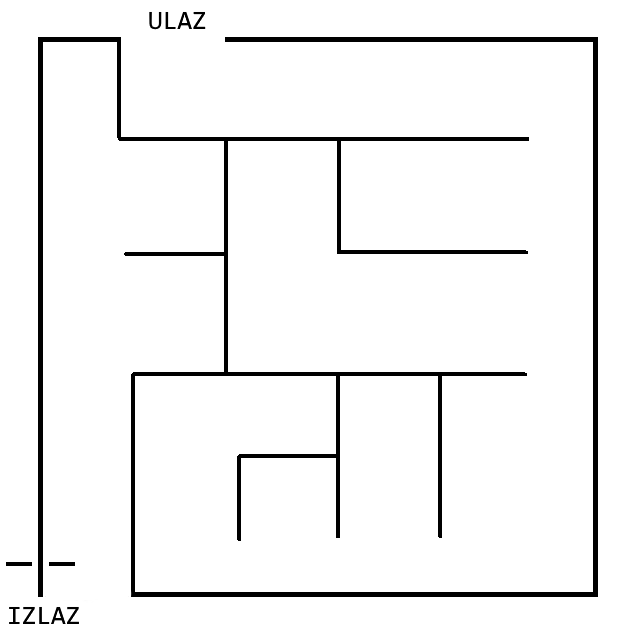
\includegraphics[scale=0.5]{maze}
Slika 1. Skica labirinta

\vspace{3mm}

Važno je uočiti da imamo dvije crte okomite na labirint koje ga ne dodiruju pri izlazu iz labirinta. Te će nam crte služiti kao znak da smo završili labirint.

\vspace{3mm}

Dakle, znamo da će robot završiti kada će mu senzori R2 i L2 biti na crnoj podlozi (pokazivat će 1).

\vspace{3mm}



"Senzor za praćenje linije nalazi se ispod robota. Sastoji se od 5 senzora, tri unutarnja (R1, M, L1) i  dva vanjska (R2 i L2), od kojih svaki ima infracrveni odašiljač i infracrveni prijemnik. Infracrveni odašiljač neprekidno emitira infracrvenu svjetlost tijekom kretanja robota. Infracrveno svjetlo se reflektira kada se robot susreće s bijelom ili nekom drugom svijetlom površinom i tada prijemnik prima infracrveni signal i upravljačkoj pločici šalje vrijednost 0. Ako se infracrveno svjetlo apsorbira ili se ne može odraziti (na tamnim površinama), prijemnik neće primiti infracrveni signal pa šalje vrijednost 1.

Kada je barem jedan od 5 senzora za praćenje linije na crnoj (tamnoj) površini, s gornje strane robota uključit će se plavi indikator. Inače je indikator isključen.

Raspon detekcije je 1 do 2 cm. Ako je robot predaleko od površine (udaljeniji od 2 centimetara), infracrveno svjetlo se ne može reflektirati pa senzor šalje vrijednost 1 kao u slučaju kad se robot nalazi na tamnoj površini." $^{[1]}$ (https://izradi.croatianmakers.hr/lessons/senzor-za-pracenje-linije-2/)

\vspace{3mm}



\section{Upute za provedbu projekta}

% -------------------------------------------------------------
% -------------------------------------------------------------
% -------------------------------------------------------------
% -------------------------------------------------------------
% -------------------------------------------------------------


\iffalse
    "Ovaj materijal je rađen tako da svaka osoba, čak i neka koja nikad nije programirala ili koristila MakeCode
    sučelje, može pratiti upute korak po korak. Svaki od ovih koraka je detaljno razrađen te također opisuje
    postupak dolaska do naredbi i njihovih promjena potrebnih za programiranje ove igre.
    Sve slike u ovom materijalu, zajedno s demonstracijskim i edukacijskim videom ovog projekta, moguće je
    pronaći u prilogu ovog materijala u punoj veličini i rezoluciji." (primjer Snake projekta)
\fi

% -------------------------------------------------------------
% -------------------------------------------------------------
% -------------------------------------------------------------
% -------------------------------------------------------------
% -------------------------------------------------------------

\subsection{Instalacija}

Micro:bit možete programirati putem Mind+ programa na osobnom računalu.

Preuzmite program na \href{https://mindplus.cc/download-en.html}{ovoj} poveznici.


\subsection{Postavljanje programa}

Nakon što ste preuzeli Mind+ program i instalirali ga na svoje računalo, pokrenite ga.

Otvaranjem programa prikazat će se prozor kao na slici. Kako biste postavili jezik programa na engleski, odaberite kotačić u gornjem desnom kutu.

\vspace{3mm}

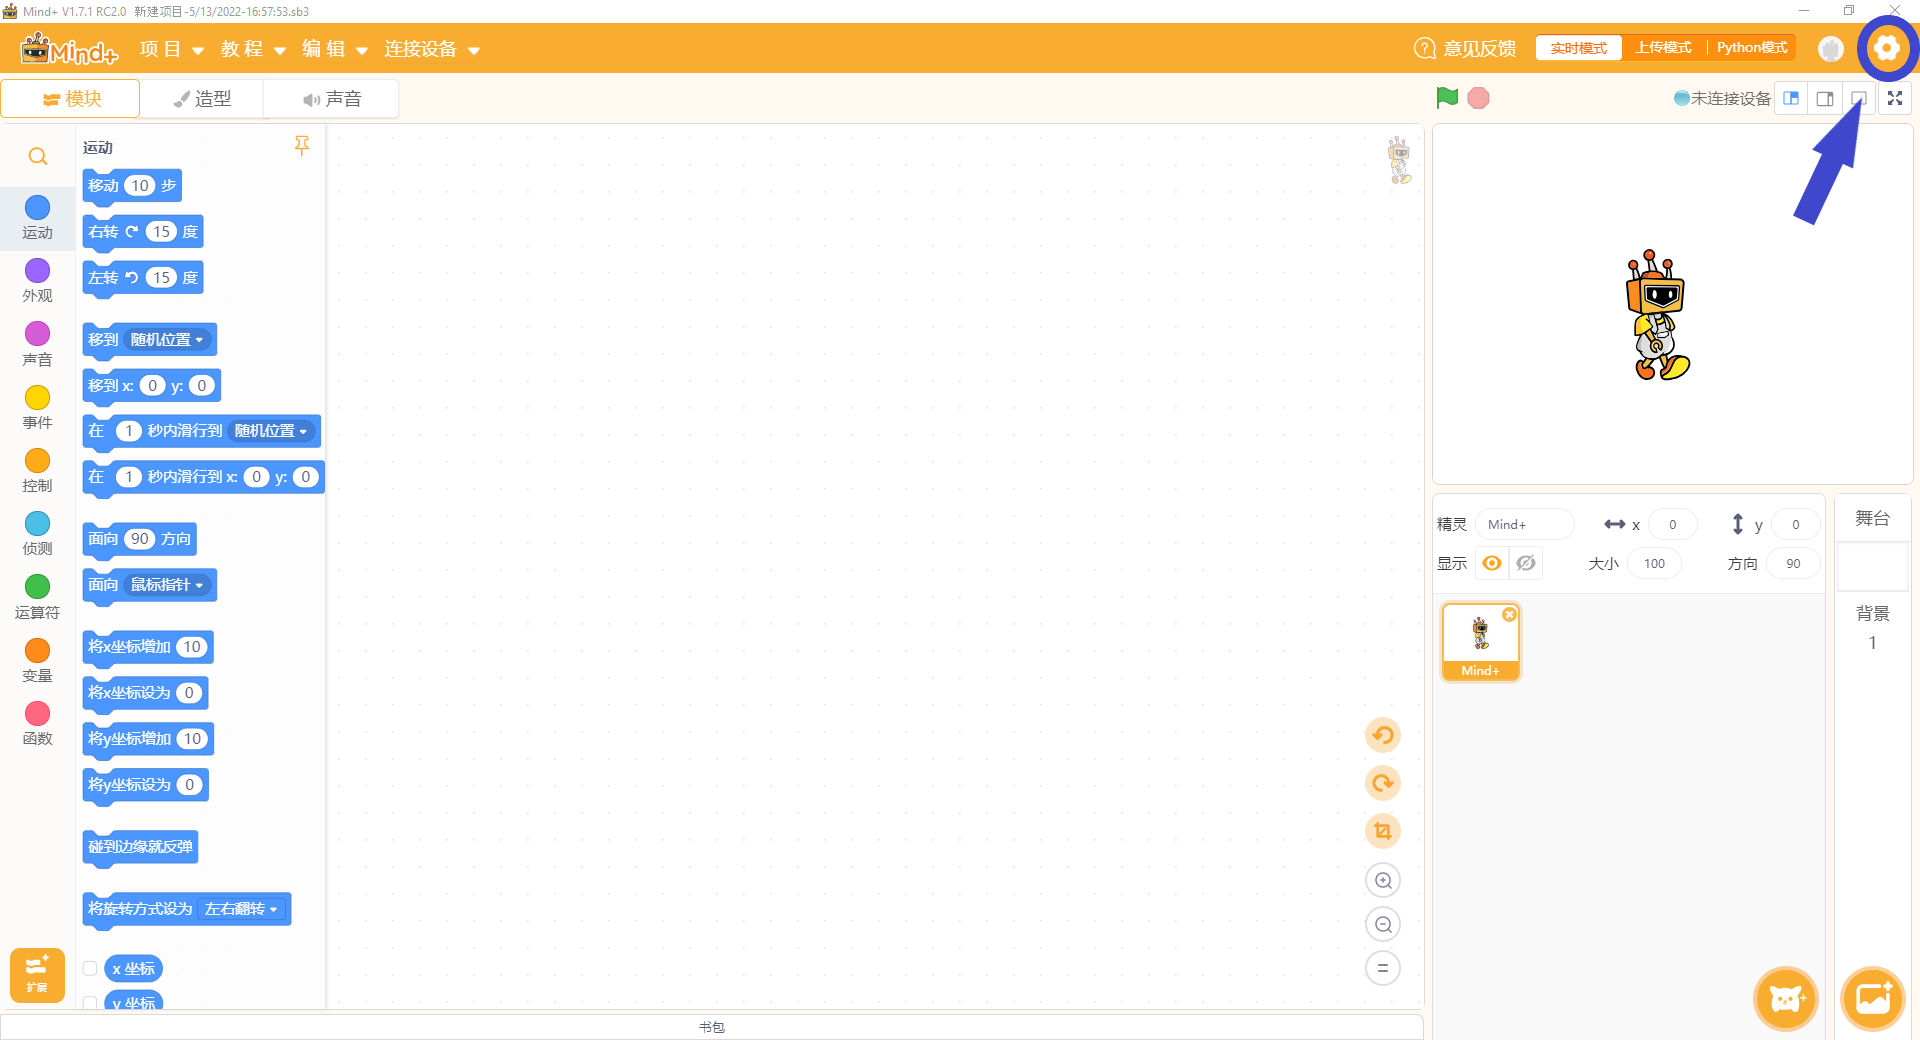
\includegraphics[scale=0.35]{Mindplus1.png}

\vspace{3mm}

Otvara se prozor kao na slici. Odaberite \textbf{English}. Prilikom svakog sljedećeg otvaranja, jezik aplikacije bit će engleski.

\vspace{3mm}

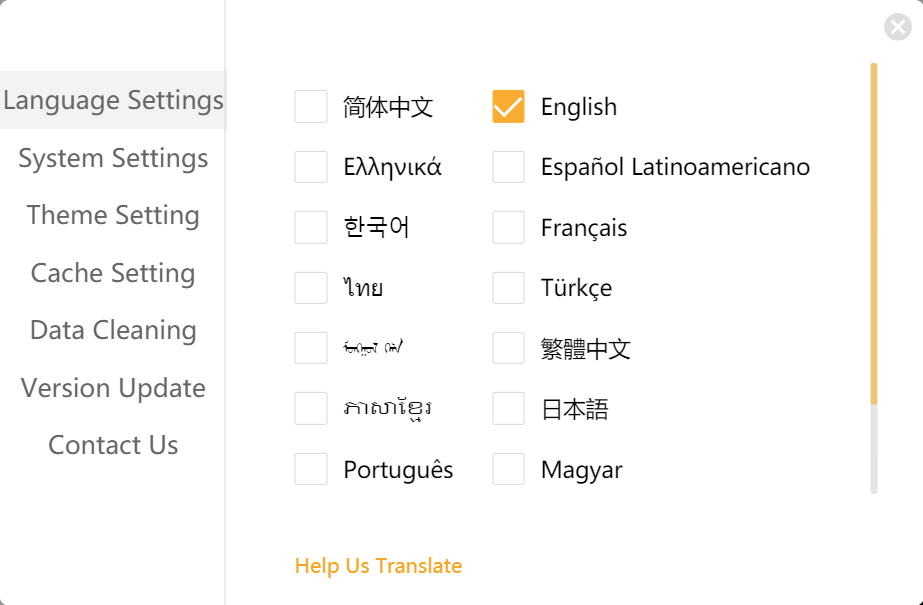
\includegraphics[scale=0.6]{Mindplus2.png}

\vspace{3mm}

Sada je potrebno postaviti način rada u \textbf{Offline} pritiskom na opciju u gornjem desnom dijelu. Nakon odabira offline načina rada, prikazuje se prozor kao na slici.

\vspace{3mm}

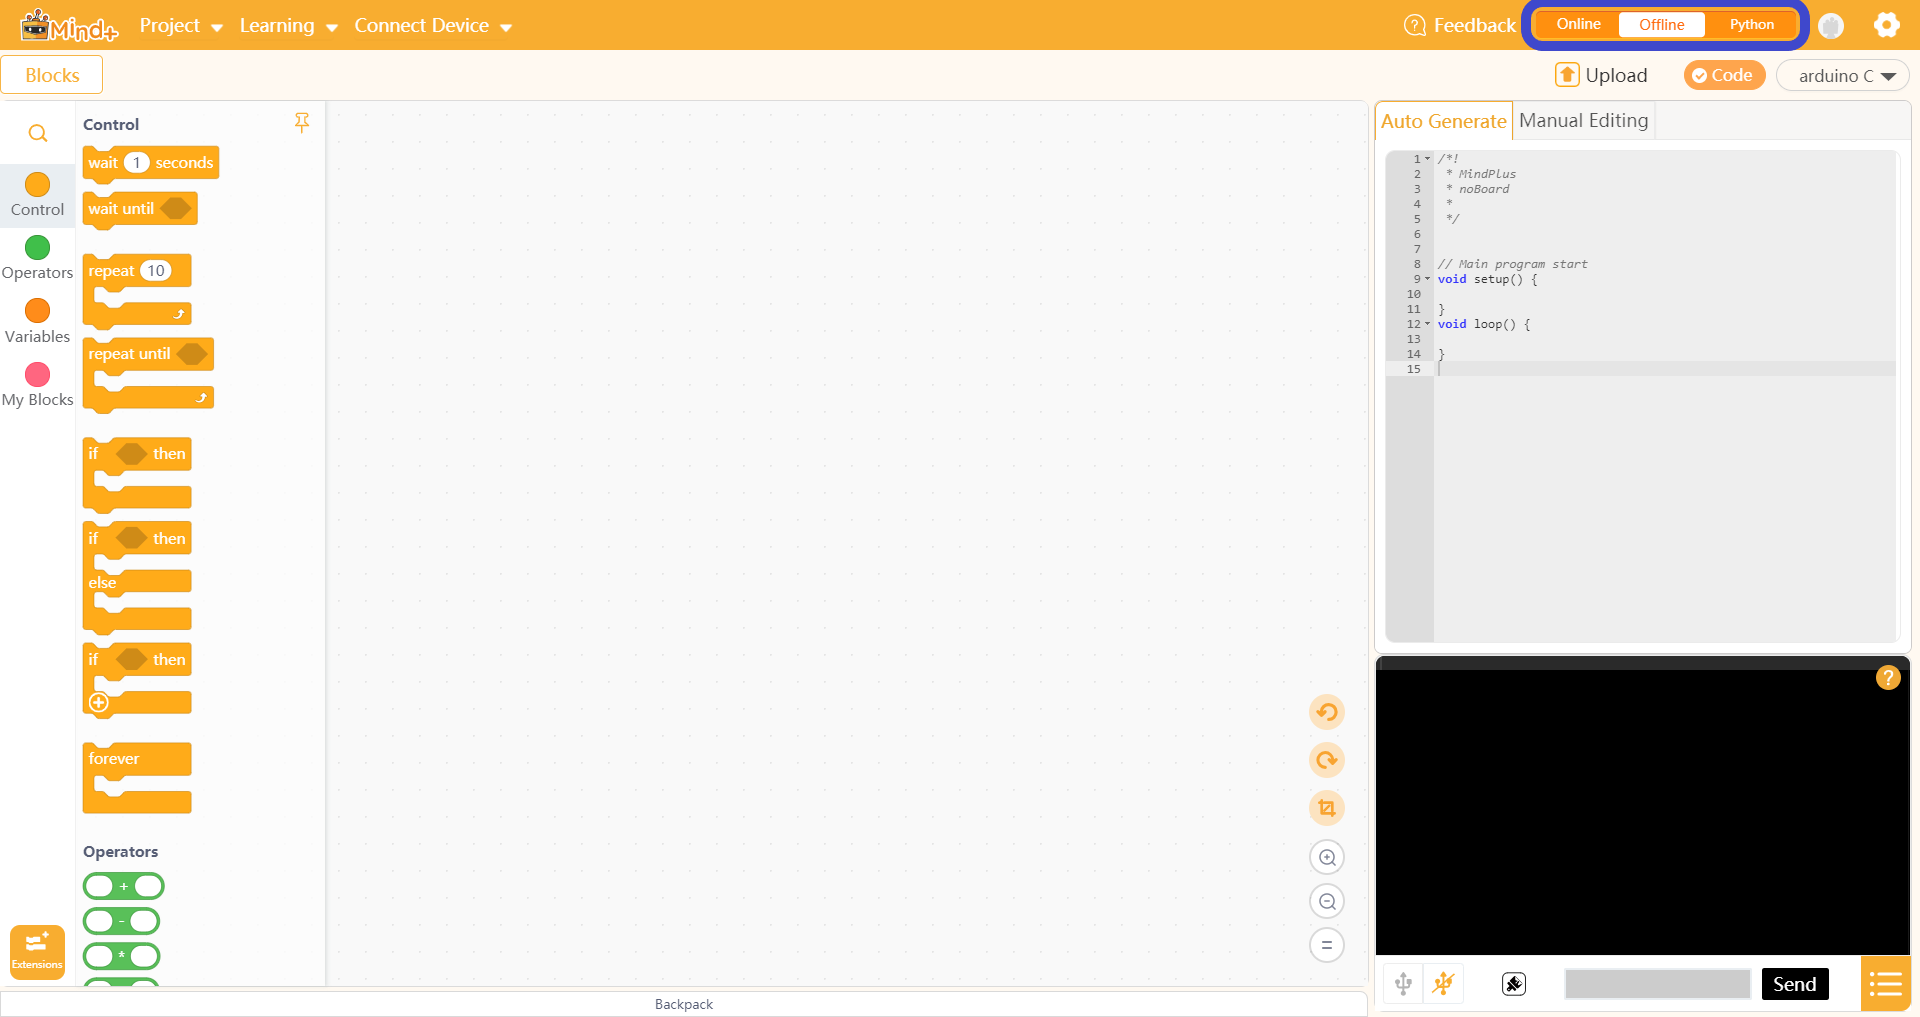
\includegraphics[scale=0.35]{Mindplus3.png}

\vspace{3mm}

Mind+ program baziran je na Scratch programskom jeziku u kojem su nadograđene komponente za programiranje micro:bita i micro:Maqueen Plus robot te je unutar Mind+ programa potrebno dodati micro:bit i micro:Maqueen Plus uređaj.

Kako biste dodali potrebne uređaje, potrebno je kliknuti na \textbf{Extensions} oznaku u donjem lijevom kutu aplikacije.

\vspace{3mm}

\includegraphics[]{Mindplus4.png}

\vspace{3mm}

Otvorit će se ploča s \textbf{Board} uređajima.

\vspace{3mm}

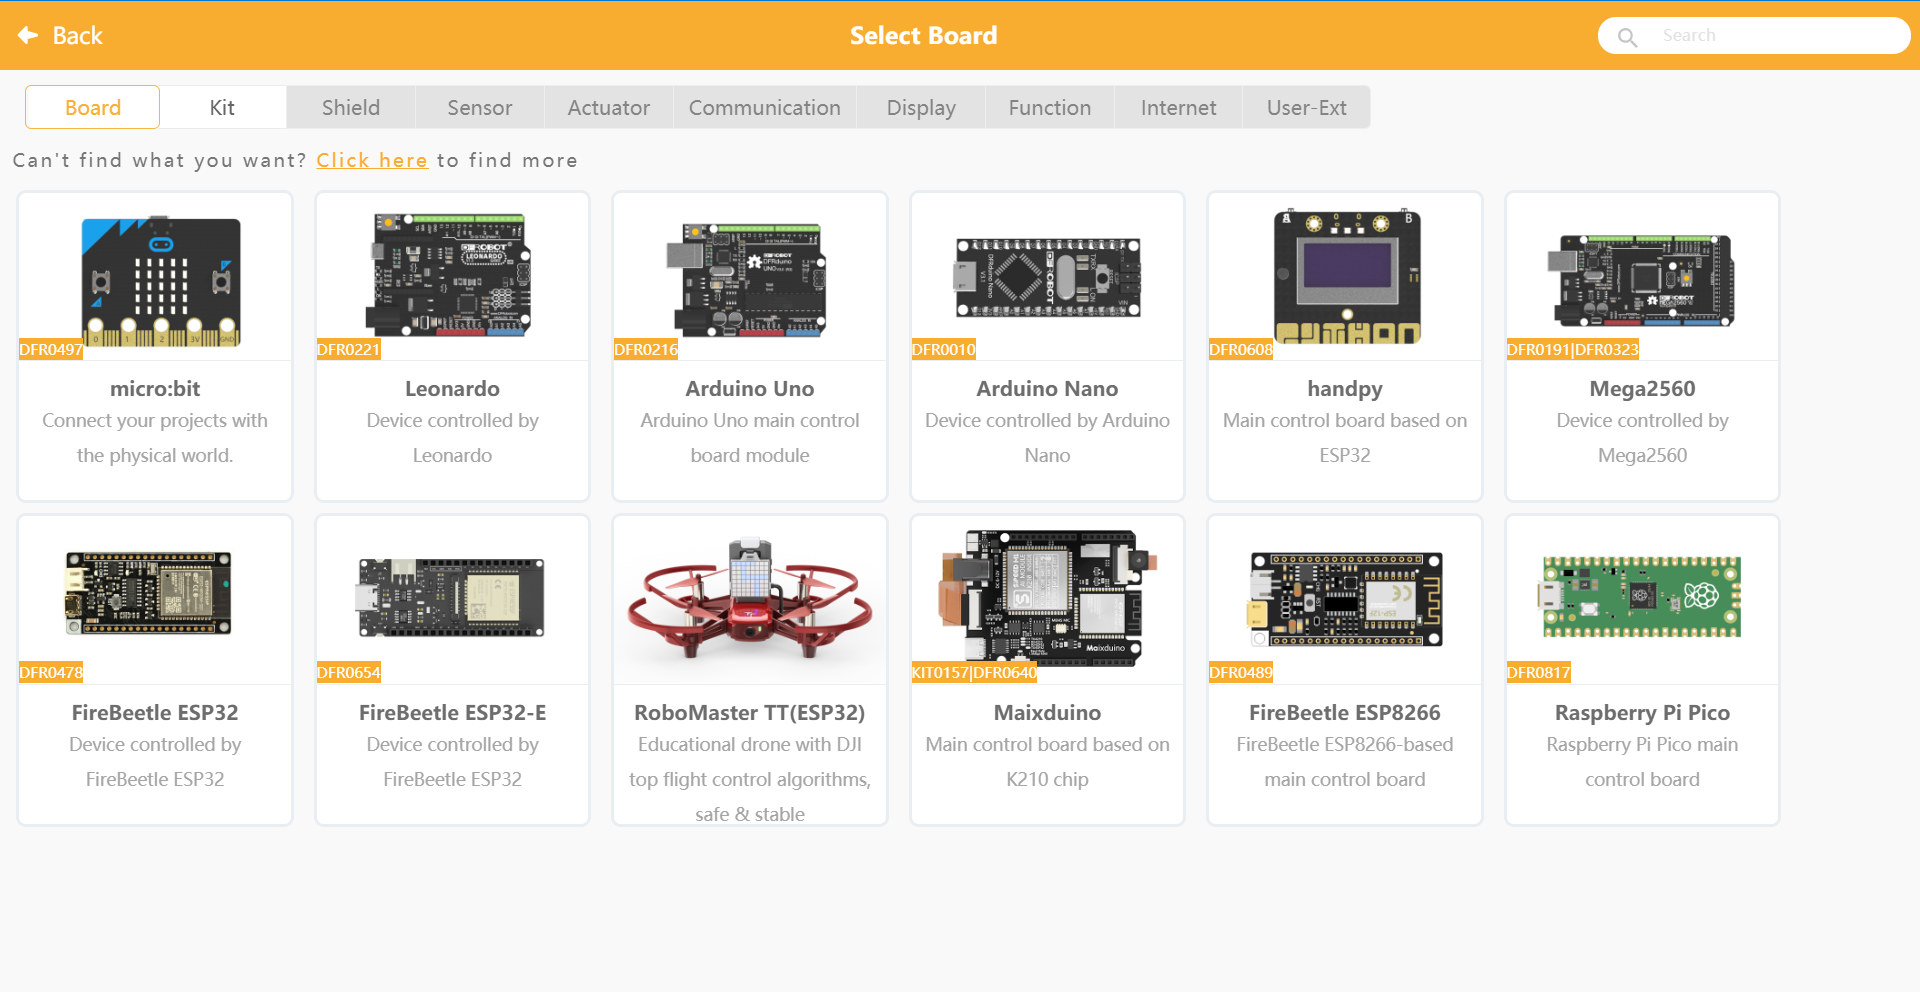
\includegraphics[scale=0.4]{Mindplus5.png}

\vspace{3mm}

U dijelu \textbf{Board} odaberite uređaj \textbf{micro:bit}.

\vspace{3mm}

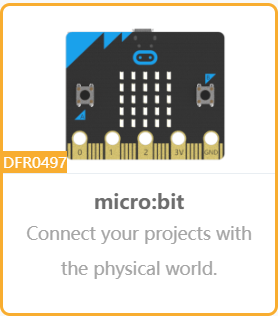
\includegraphics[scale=0.6]{Mindplus6.png}

\vspace{3mm}

Nakon što odaberete micro:bit, otvorite \textbf{Shield} proširenja.

\vspace{3mm}

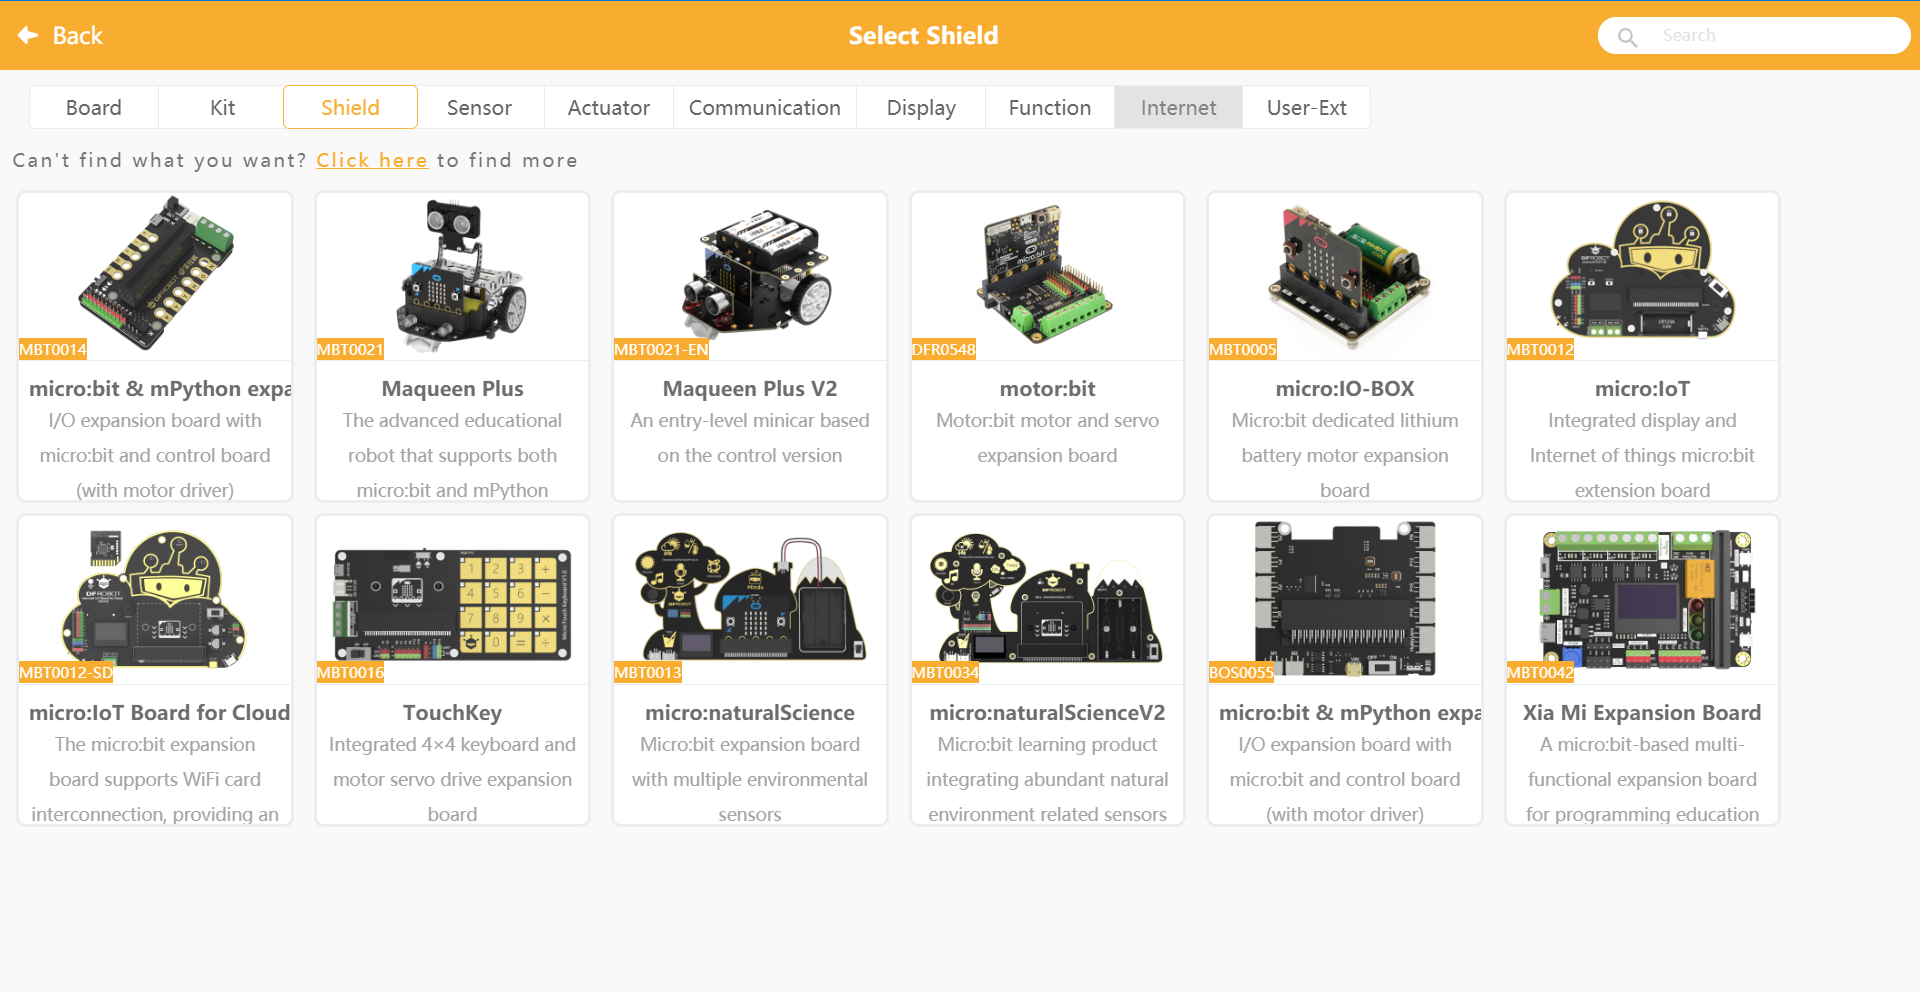
\includegraphics[scale=0.4]{Mindplus7.png}

\vspace{3mm}

U \textbf{Shield} dijelu odaberite uređaj \textbf{Maqueen Plus V2}.

\vspace{3mm}

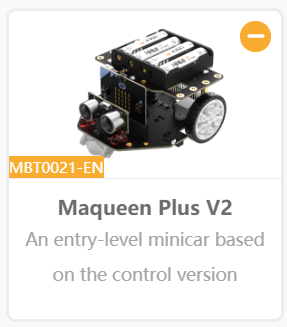
\includegraphics[scale=0.6]{Mindplus8.png}

\vspace{3mm}

Sada opcijom \textbf{Back} izađite iz ploče s proširenjima.

\vspace{3mm}

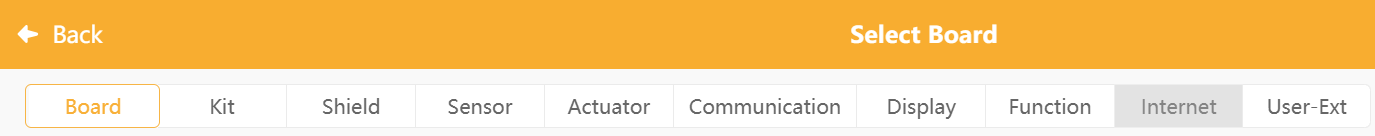
\includegraphics[scale=0.5]{Mindplus9.png}

\vspace{3mm}

Time ćete se vratiti u editor za programiranje te ćete u popisu kategorija pronaći dvije nove kategorije - \textbf{micro:bit} i \textbf{Expansion Board}. U kategoriji \textbf{micro:bit} nalaze se naredbe za programiranje rada micro:bita, a u kategoriji \textbf{Expansion Board} za programiranje rada robota. Ovaj korak treba napraviti svaki put kada otvorite Mind+.


\vspace{3mm}

\hspace*{10mm}
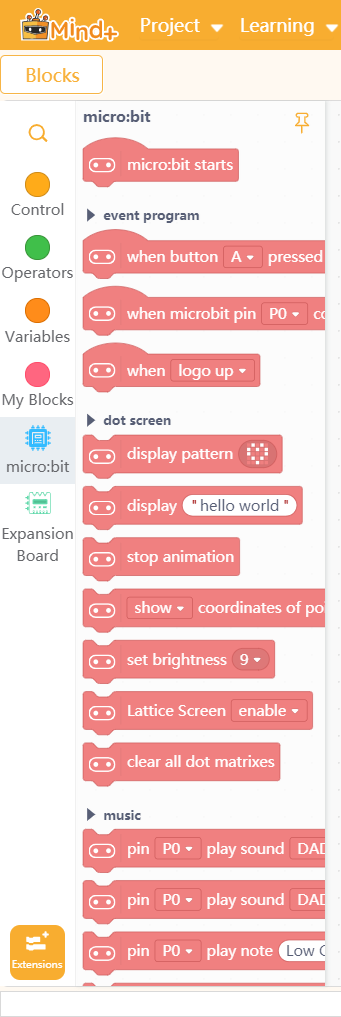
\includegraphics[scale=0.55]{Mindplus10.png}
\hspace*{40mm}
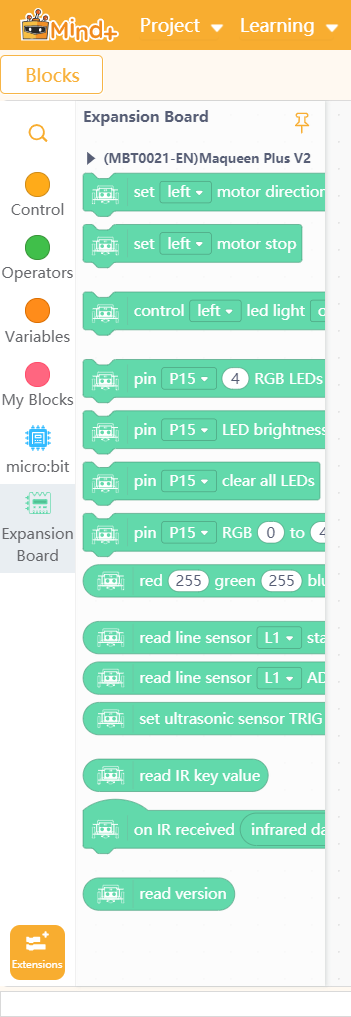
\includegraphics[scale=0.55]{Mindplus11.png}

\vspace{3mm}


\subsection{Povezivanje micro:bita s aplikacijom}

Sada možete putem USB kabla povezati micro:bit s računalom.

U dijelu \textbf{Connect Device} pojavit će se naziv porta na kojem je spojen micro:bit na računalu. Odaberite taj port.

\vspace{3mm}

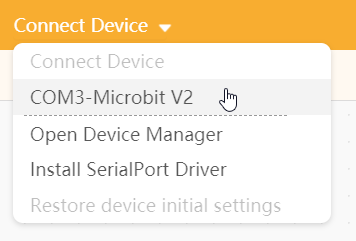
\includegraphics[scale=0.75]{Mindplus12.png}

\vspace{3mm}

Sada je micro:bit povezan s Mind+ aplikacijom.



\section{Rješavanje zadatka}

Za rješavanje zadatka potrebne su 3 numeričke varijable: gotovo, rjesava i vrijeme. Za dodavanje tih varijabli pritisnite \textbf{Variables} te nakon toga pritisnite \textbf{Make a Numeric Variable}.

\vspace{3mm}

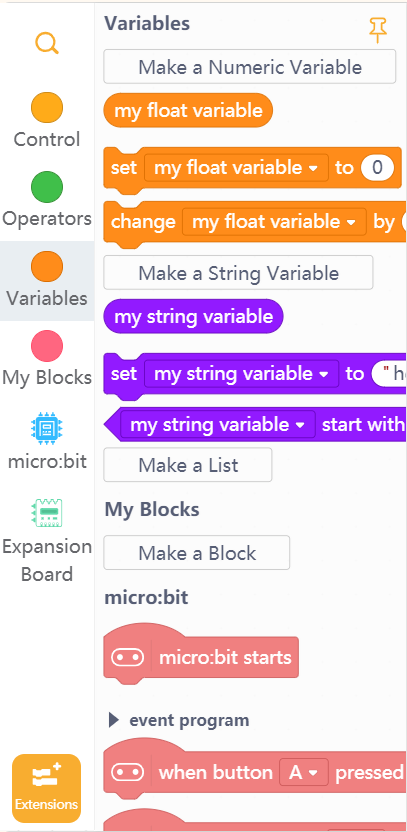
\includegraphics[scale=0.75]{Rjesenje1.png}

\vspace{3mm}

Pojavit će se prozor u koji upišite \textbf{gotovo} te pritisnite na \textbf{OK}.

\vspace{3mm}

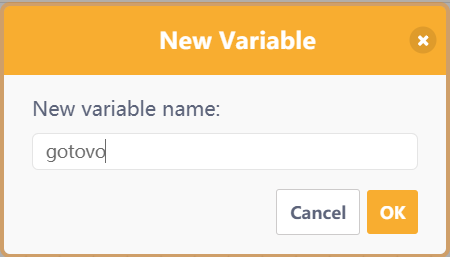
\includegraphics[scale=0.75]{Rjesenje2.png}

\vspace{3mm}

Isti postupak kako biste stvorili varijable \textbf{rjesava} i \textbf{vrijeme}.

Varijabla \textbf{gotovo} je 1 ako je robot prošao kroz labirint, a inače 0 te se njena vrijednost može mijenjati pritiskom na gumb B.

Varijabla \textbf{rjesava} je 1 ako robot trenutno pokušava riješiti labirint, a inače 0 te se njena vrijednost može mijenjati pritiskom na gumb A.

Varijabla \textbf{vrijeme} služi za brojanje vremena rješavanja labirinta.

Za promjenu varijable \textbf{gotovo} na pritisak gumba B pritisnite \textbf{My Blocks} te pod \textbf{event program} povucite \textbf{when button A pressed} na sredinu programa.

\vspace{3mm}

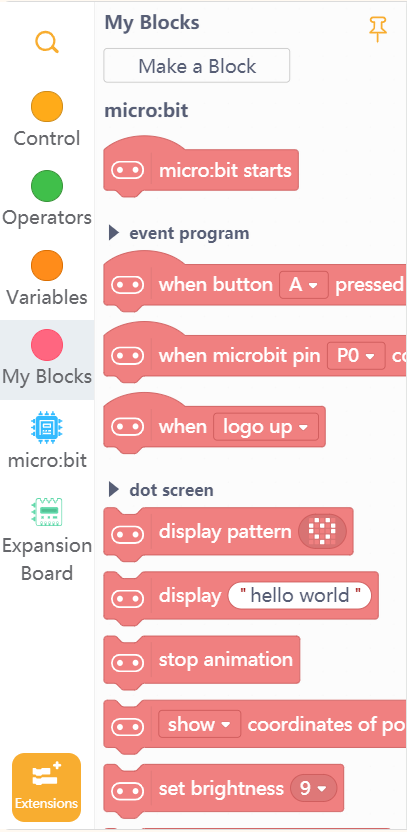
\includegraphics[scale=0.75]{Rjesenje3.png}

\vspace{3mm}

Zatim pritisnite na \textbf{A} i u padajućem izborniku odaberite B.

\vspace{3mm}

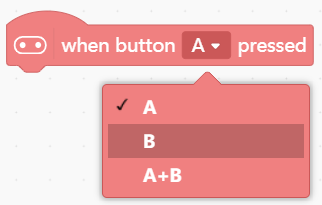
\includegraphics[scale=0.75]{Rjesenje4.png}

\vspace{3mm}

Nakon toga dodajte idući if else blok naredbi:

\vspace{3mm}

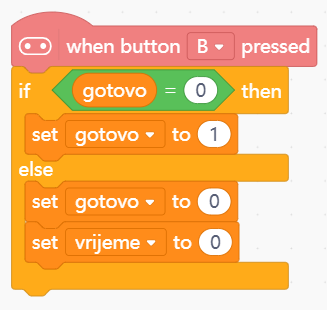
\includegraphics[scale=0.75]{Rjesenje5.png}

\vspace{3mm}

Ovaj dio programa mijenja vrijednost varijable \textbf{gotovo} i ako je dosad vrijednost bila 1, tj. ako je labirint bio riješen, vraća vrijednost varijable \textbf{vrijeme} na 0.

Dodajte sličan blok naredbi za pritisak na gumb A:

\vspace{3mm}

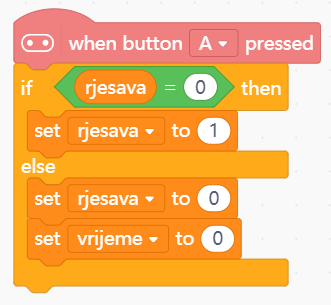
\includegraphics[scale=0.75]{Rjesenje6.png}

\vspace{3mm}

Nakon toga između \textbf{micro:bit starts} i \textbf{forever} bloka dodajte naredbe za postavljanje svih varijabli na 0:

\vspace{3mm}

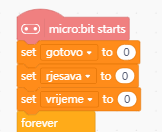
\includegraphics[scale=0.75]{Rjesenje7.png}

\vspace{3mm}

Zatim unutar \textbf{forever} bloka dodajte

\vspace{3mm}

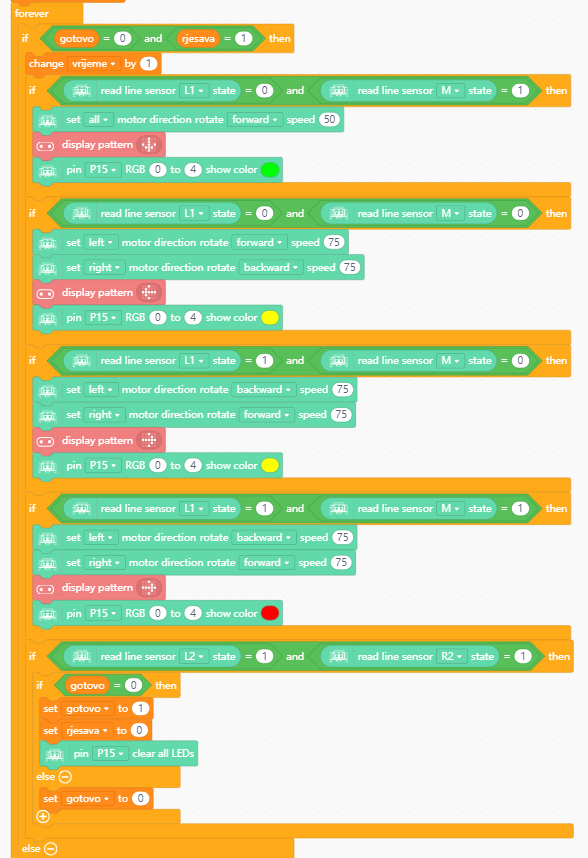
\includegraphics[scale=0.75,width=\textwidth]{Rjesenje8.png}
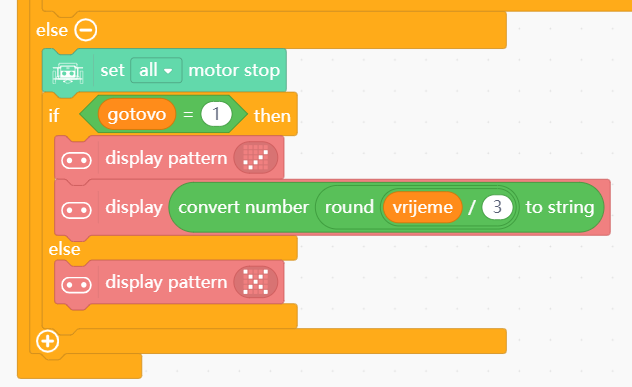
\includegraphics[scale=0.75]{Rjesenje9.png}

\vspace{3mm}

Ovaj kod radi sljedeće:

\begin{itemize}
    \item ako robot nije našao izlaz iz labirinta i pokušava ga riješiti:
    \begin{itemize}
        \item ako se senzor L1 lijevo od crte, a senzor M na crti, prati crtu, svijetli zelenom bojom i na ekranu je prikazana strelica ↑
        \item ako se oba senzora L1 i M nalaze lijevo od crte robot skreće udesno, svijetli žutom bojom i na ekranu je prikazana strelica →
        \item ako se senzor L1 na crti, a senzor M desno od crte, prati crtu, svijetli žutom bojom i na ekranu je prikazana strelica ←
        \item ako se oba senzora L1 i M nalaze na crti robot skreće ulijevo, svijetli crvenom bojom i na ekranu je prikazana strelica ←
        \item ako se oba senzora L2 i R2 nalaze na crti robot skreće robot je došao do kraja labirinta pa mijenja varijabla gotovo i gasi LED-lampica
    \end{itemize}
    (strelice na displayu su zrcaljene su u odnosu na ove u uputama kako bi izgledale dobro kada se gleda na robot sprijeda)
    \item inače:
    \begin{itemize}
        \item ako je labirint riješen robot na displayu prikazuje kvačicu i vrijeme rješavanja u sekundama
        \item inače prikazuje x
    \end{itemize}
\end{itemize}



\subsection{Prebacivanje koda na robot}

Nakon postavljanja svih blokova, pritisnite na gumb \textbf{Upload} kako biste prenijeli kod na robot.

\vspace{3mm}

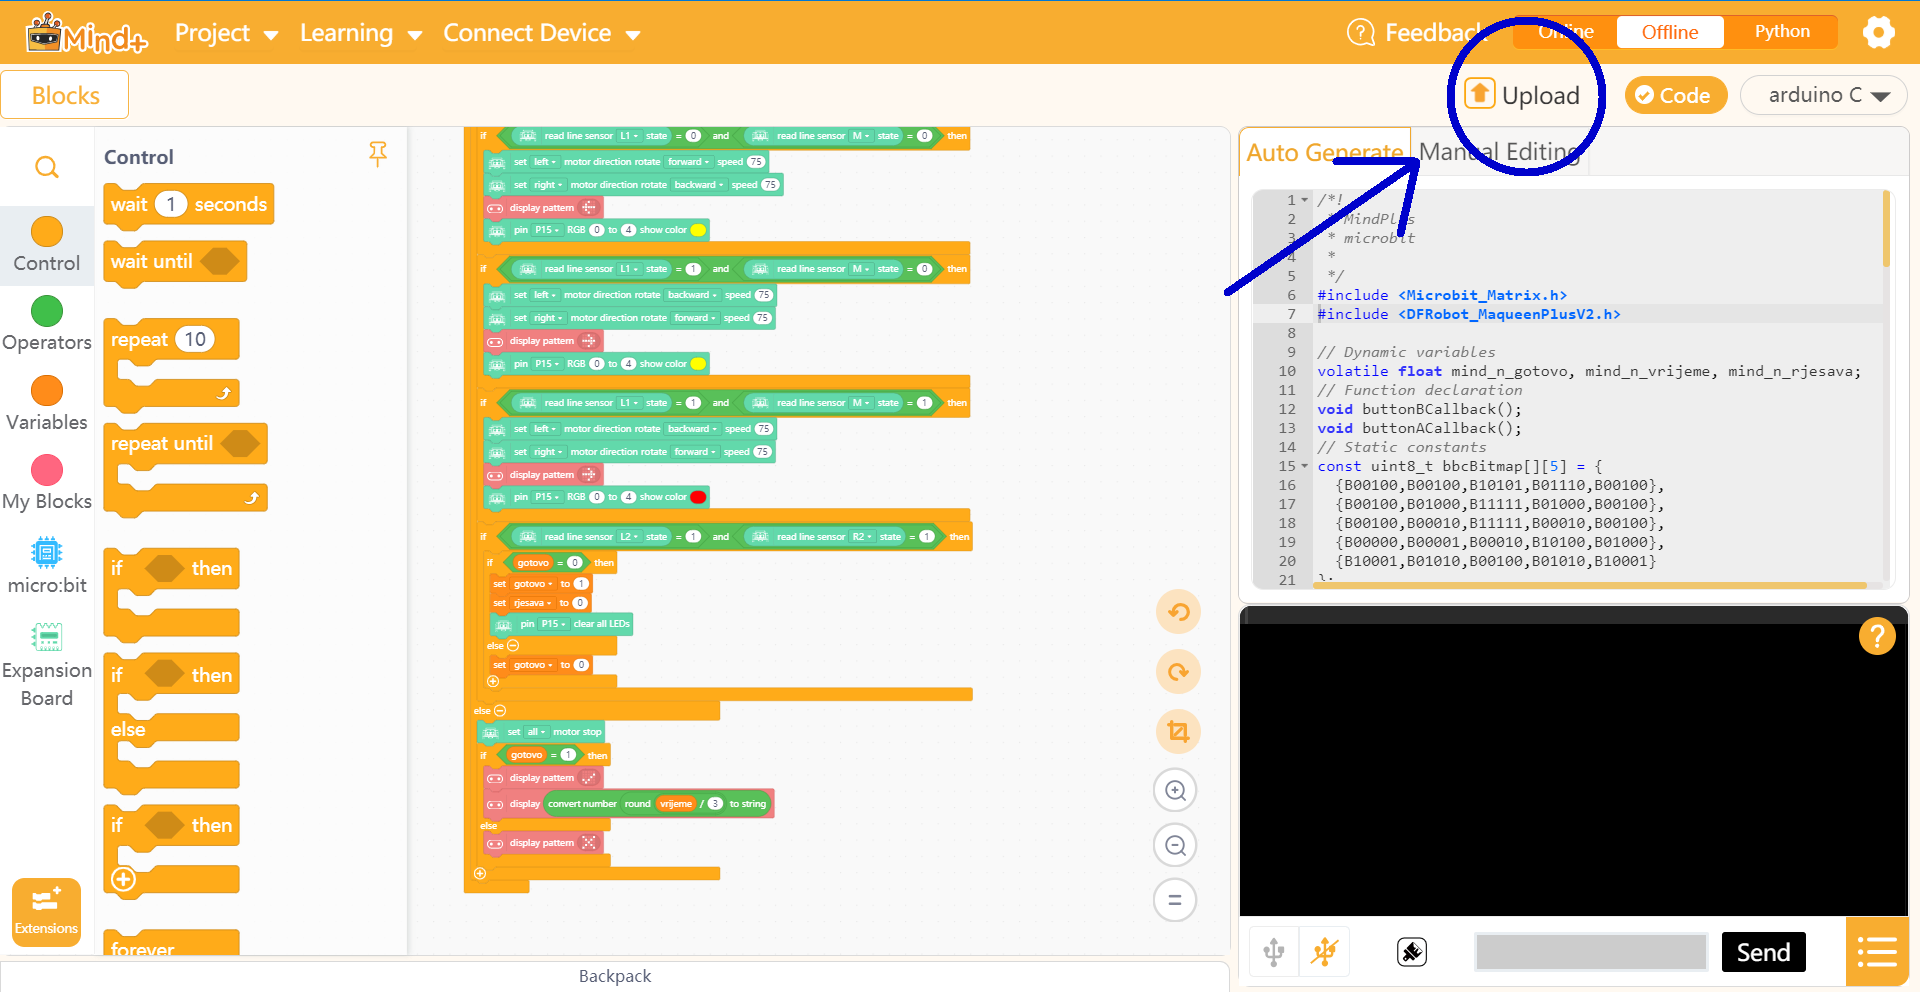
\includegraphics[scale=0.3]{Rjesenje10.png}

% -------------------------------------------------------------
% -------------------------------------------------------------
% -------------------------------------------------------------
% -------------------------------------------------------------
% -------------------------------------------------------------

\iffalse
    *SLIKE*

\subsection{Algoritam za praćenje desnog zida}


Trebamo 1 if else i 5 if then blokova koji provjeravaju 6 mogućih očitanja senzora za praćenje linije te ovisno o njima određuju smjer kretanja robota.

Ako su svi senzori na svijetloj podlozi (if read line sensor L2 state = 0 and sensor L1 state = 0 and read line sensor M state = 0 and read line sensor R1 state = 0 and read line sensor R2 state = 0) robot je došao do kraja labirinta i zaustavljamo sve motore. Inače, provjeravamo očitanja senzora.

Ako su svi senzori na tamnoj podlozi (if read line sensor L2 state = 1 and sensor L1 state = 1 and read line sensor M state = 1 and read line sensor R1 state = 1 and read line sensor R2 state = 1) robot se kreće ravno.

"Ako je senzor L1 na svijetloj podlozi i senzor M na tamnoj podlozi (if read line sensor L1 state = 0 and read line sensor M state = 1) robot se kreće ravno (set all motor direction rotate forward speed 50).

Ako su oba senzora na svijetloj podlozi (if read line sensor L1 state = 0 and read line sensor M state = 0), robot skretanjem u desno traži tamnu podlogu kako bi došao u situaciju da vrijednost senzora M bude 1 i da robot nastavi s vožnjom naprijed.

U situacijama kad je robot s L1 senzorom na tamnoj, a s M senzorom na svijetloj podlozi (if read line sensor L1 state = 1 and read line sensor M state = 0) ili s oba senzora na tamnoj podlozi (if read line sensor L1 state = 1 and read line sensor M state = 1), robot skretanjem ulijevo dolazi do položaja iz prve situacije gdje se kreće ravno." $^{[2]}$ (https://izradi.croatianmakers.hr/lessons/pracenje-linije-s-vanjske-strane/)

Gotovi kod bi trebao izgledati ovako:

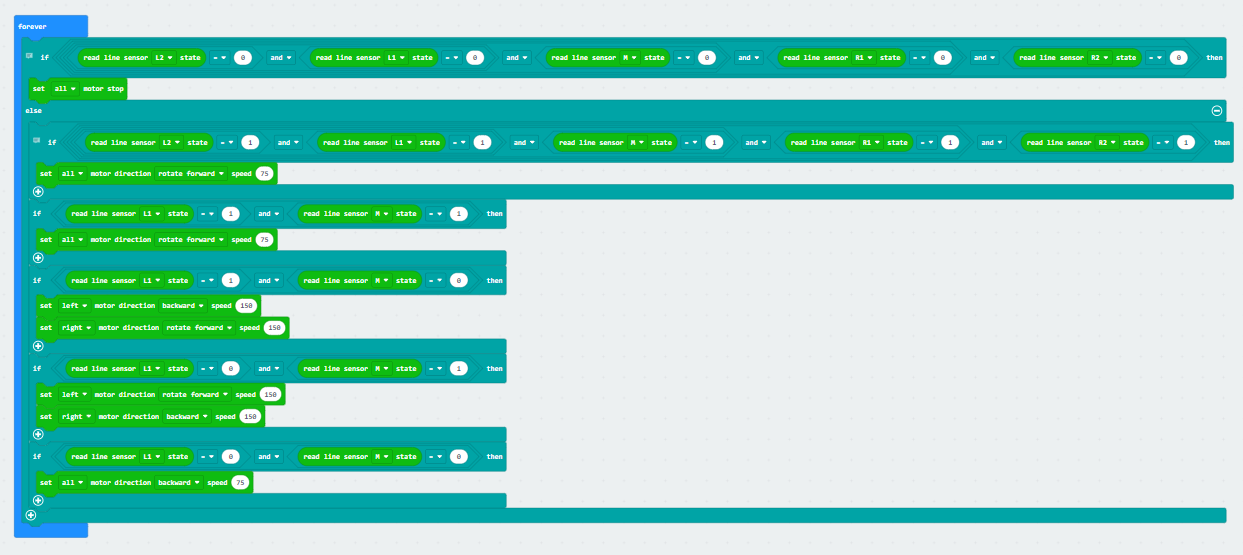
\includegraphics[scale=0.6]{pracenje-desnog-zida}

Slika 2. Kod za praćenje desnog zida

    \section{(DODATNO) *Složeniji algoritam za prolazak labirinta*}

    \section{(DODATNO) Generacija labirinta}
\fi

\end{document}